% When submitting your files, remember to upload this *tex file, the pdf generated with it, the *bib file (if bibliography is not within the *tex) and all the figures.
%%%%%%%%%%%%%%%%%%%%%%%%%%%%%%%%%%%%%%%%%%%%%%%%%%%%%%%%%%%%%%%%%%%%%%%%%%%%%%%%%%%%%%%%%%%%%%%%%%%%%%%%%%%%%%%%%%%%%%%%%%%%%%%%%%%%%%%%%%%%%%%%%%%%%%%%%%%

%%% Version 3.4 Generated 2018/06/15 %%%
%%% You will need to have the following packages installed: datetime, fmtcount, etoolbox, fcprefix, which are normally inlcuded in WinEdt. %%%

\documentclass[utf8]{FrontiersinVancouver}

\usepackage{url,hyperref,lineno,microtype,subcaption}
\usepackage[onehalfspacing]{setspace}
\usepackage[footnotes,definitionLists,hashEnumerators,smartEllipses,hybrid,citations]{markdown}

\linenumbers


% Leave a blank line between paragraphs instead of using \\


\def\keyFont{\fontsize{8}{11}\helveticabold }
\def\firstAuthorLast{Sample {et~al.}} %use et al only if is more than 1 author
\def\Authors{Steve Harris\,$^{1,2*}$ Tim Bonnici\,$^{1,2}$ Thomas Keen\,$^{1}$ Watjana Lilaonitkul\,$^{1}$ Mark J White\,$^{4}$ Nel Swanepoel\,$^{3}$ }
% Affiliations should be keyed to the author's name with superscript numbers and be listed as follows: Laboratory, Institute, Department, Organization, City, State abbreviation (USA, Canada, Australia), and Country (without detailed address information such as city zip codes or street names).
% If one of the authors has a change of address, list the new address below the correspondence details using a superscript symbol and use the same symbol to indicate the author in the author list.

\def\Address{$^{1}$Institute of Health Informatics, University College London, London, UK \\
$^{2}$Department of Critical Care, University College London Hospital, London, UK  \\
$^{3}$Centre for Advanced Research Computing, University College London, London, UK \\
$^{4}$Digital Healthcare, University College London Hospital, London, UK   }

% The Corresponding Author should be marked with an asterisk
% Provide the exact contact address (this time including street name and city zip code) and email of the corresponding author
\def\corrAuthor{Corresponding Author}

\def\corrEmail{steve.harris@ucl.ac.uk}






\begin{document}
\onecolumn
\firstpage{1}

\title[Translational Digital Medicine]{The Five Pillars of Translational Digital Medicine} 

\author[\firstAuthorLast ]{\Authors} %This field will be automatically populated
\address{} %This field will be automatically populated
\correspondance{} %This field will be automatically populated

\extraAuth{}% If there are more than 1 corresponding author, comment this line and uncomment the next one.
%\extraAuth{corresponding Author2 \\ Laboratory X2, Institute X2, Department X2, Organization X2, Street X2, City X2 , State XX2 (only USA, Canada and Australia), Zip Code2, X2 Country X2, email2@uni2.edu}


\maketitle
\begin{abstract}

%%% Leave the Abstract empty if your article does not require one, please see the Summary Table for full details.
\section{}
\markdownInput{00-abstract.md}


\tiny
 \keyFont{ \section{Keywords:} translational medicine, machine learning, health informatics, ml-ops, safety, artificial intelligence} 
 %All article types: you may provide up to 8 keywords; at least 5 are mandatory.
 
\end{abstract}

% \markdownInput{01-main.md}
\markdownInput{01-intro.md}
\markdownInput{02-real-world-development.md}
\markdownInput{03-ml-ops.md}
\markdownInput{04-responsible-ai.md}
\markdownInput{05-implementation.md}
\markdownInput{06-continuous-evaluation.md}
\markdownInput{08-discussion.md}







\section*{Conflict of Interest Statement}
%All financial, commercial or other relationships that might be perceived by the academic community as representing a potential conflict of interest must be disclosed. If no such relationship exists, authors will be asked to confirm the following statement: 

The authors declare that the research was conducted in the absence of any commercial or financial relationships that could be construed as a potential conflict of interest.

\section*{Author Contributions}
All authors listed have made a substantial, direct and intellectual contribution to the work, and approved it for publication.

\section*{Funding}

SH is supported by a Health Foundation Improvement Science Fellowship, and by funding from  the Biomedical Research Centre based at the University College Hospitals (UCLH) National Health Service (NHS) Foundation Trust and University College London (UCL). NS is supported by funding from Health Data Research UK. SH, TK, and NS are supported funds from the National Institute for Health Research (Artificial Intelligence, Digitally adapted, hyper-local real-time bed forecasting to manage flow for NHS wards, AI AWARD01786) and NHS-X.  WL is supported by a UKRI Ernest Rutherford Fellowship.
The views expressed in this publication are those of the author(s) and not necessarily those of the National Institute for Health Research, NHS-X or the Department of Health and Social Care.


\bibliographystyle{Frontiers-Vancouver} 
\bibliography{refs}

%%% Make sure to upload the bib file along with the tex file and PDF
%%% Please see the test.bib file for some examples of references

\section*{Figure captions}

%%% Please be aware that for original research articles we only permit a combined number of 15 figures and tables, one figure with multiple subfigures will count as only one figure.
%%% Use this if adding the figures directly in the mansucript, if so, please remember to also upload the files when submitting your article
%%% There is no need for adding the file termination, as long as you indicate where the file is saved. In the examples below the files (logo1.eps and logos.eps) are in the Frontiers LaTeX folder
%%% If using *.tif files convert them to .jpg or .png
%%%  NB logo1.eps is required in the path in order to correctly compile front page header %%%

\begin{figure}[h!]
\begin{center}
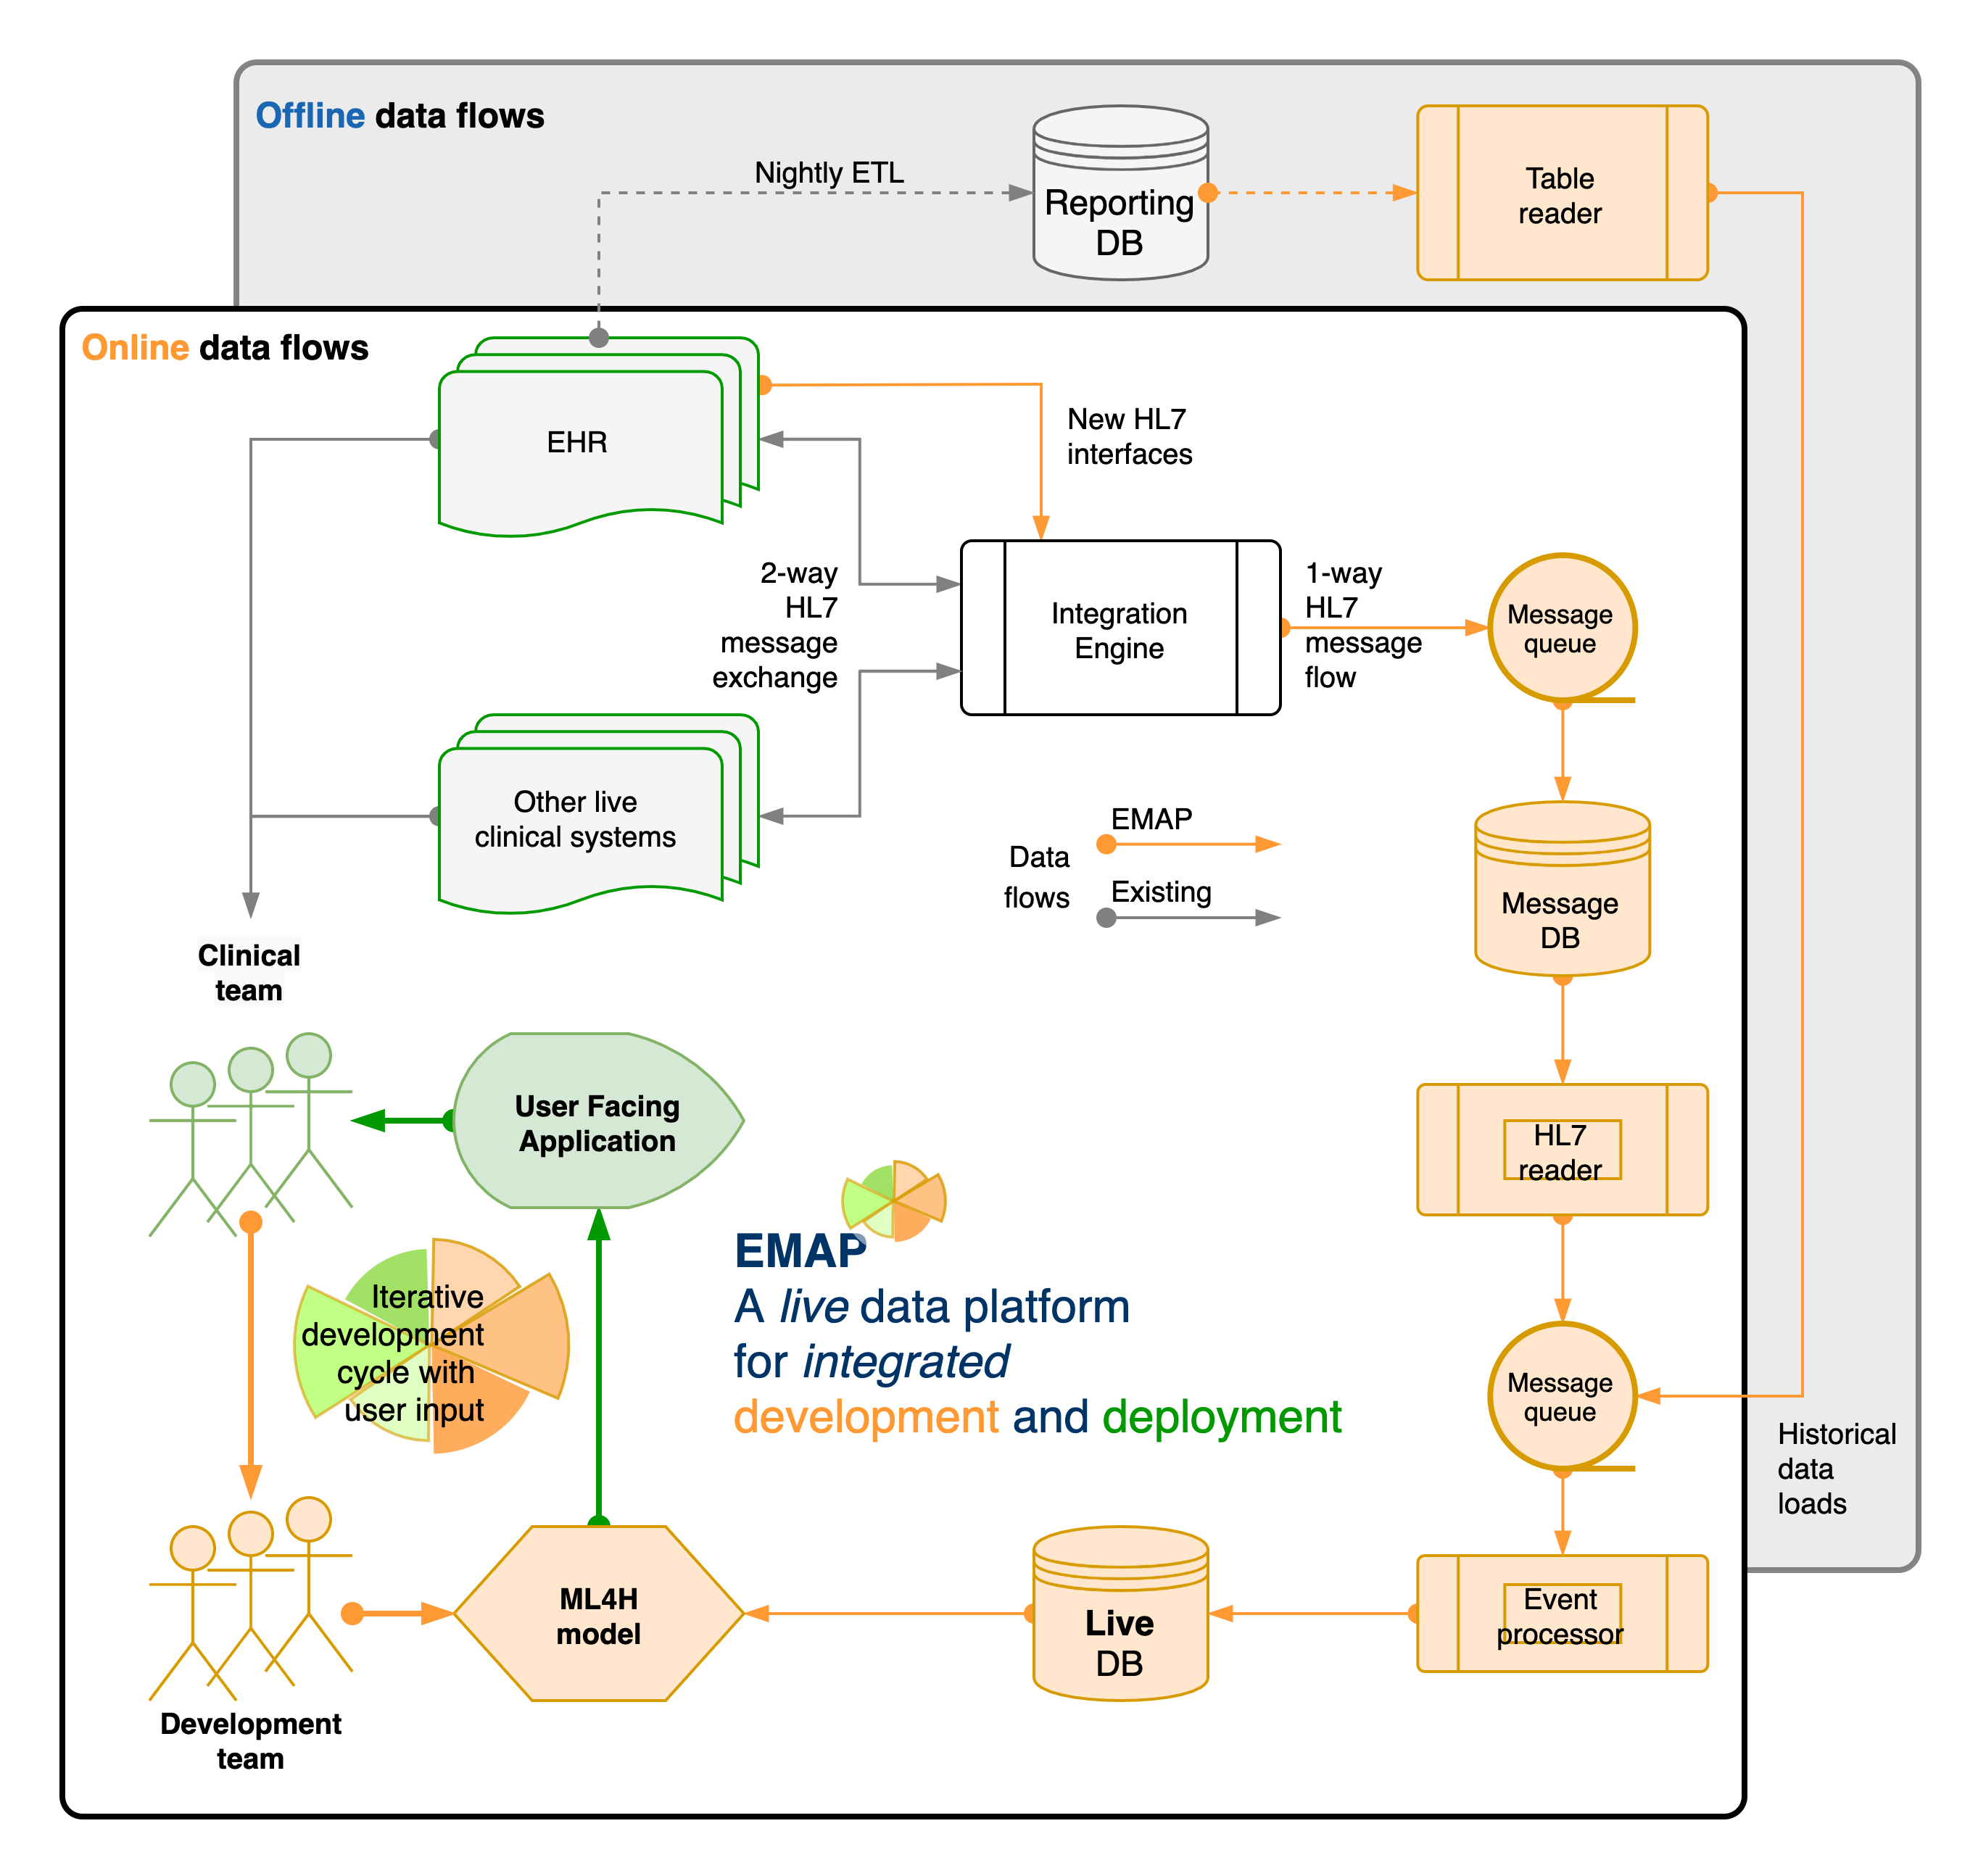
\includegraphics[width=10cm]{figs/emap.png}% This is a *.eps file
\end{center}
\caption{ 
Our real-world development is performed on the  Experimental Medicine Application Platform (EMAP). EMAP is a clinical laboratory within which ML4H researchers can iteratively build, test and gather feedback from the bedside. It unifies the data and the tools for off-line and online development of ML4H models. In brief, EMAP builds a patient orientated SQL database from HL7 version 2 (HL7v2) messages that are being exchanged between hospital systems. HL7v2 messages are ubiquitous in health care, and the \textit{de facto} standard for internal communication.
}\label{fig:1}
\end{figure}


\begin{figure}[h!]
\begin{center}
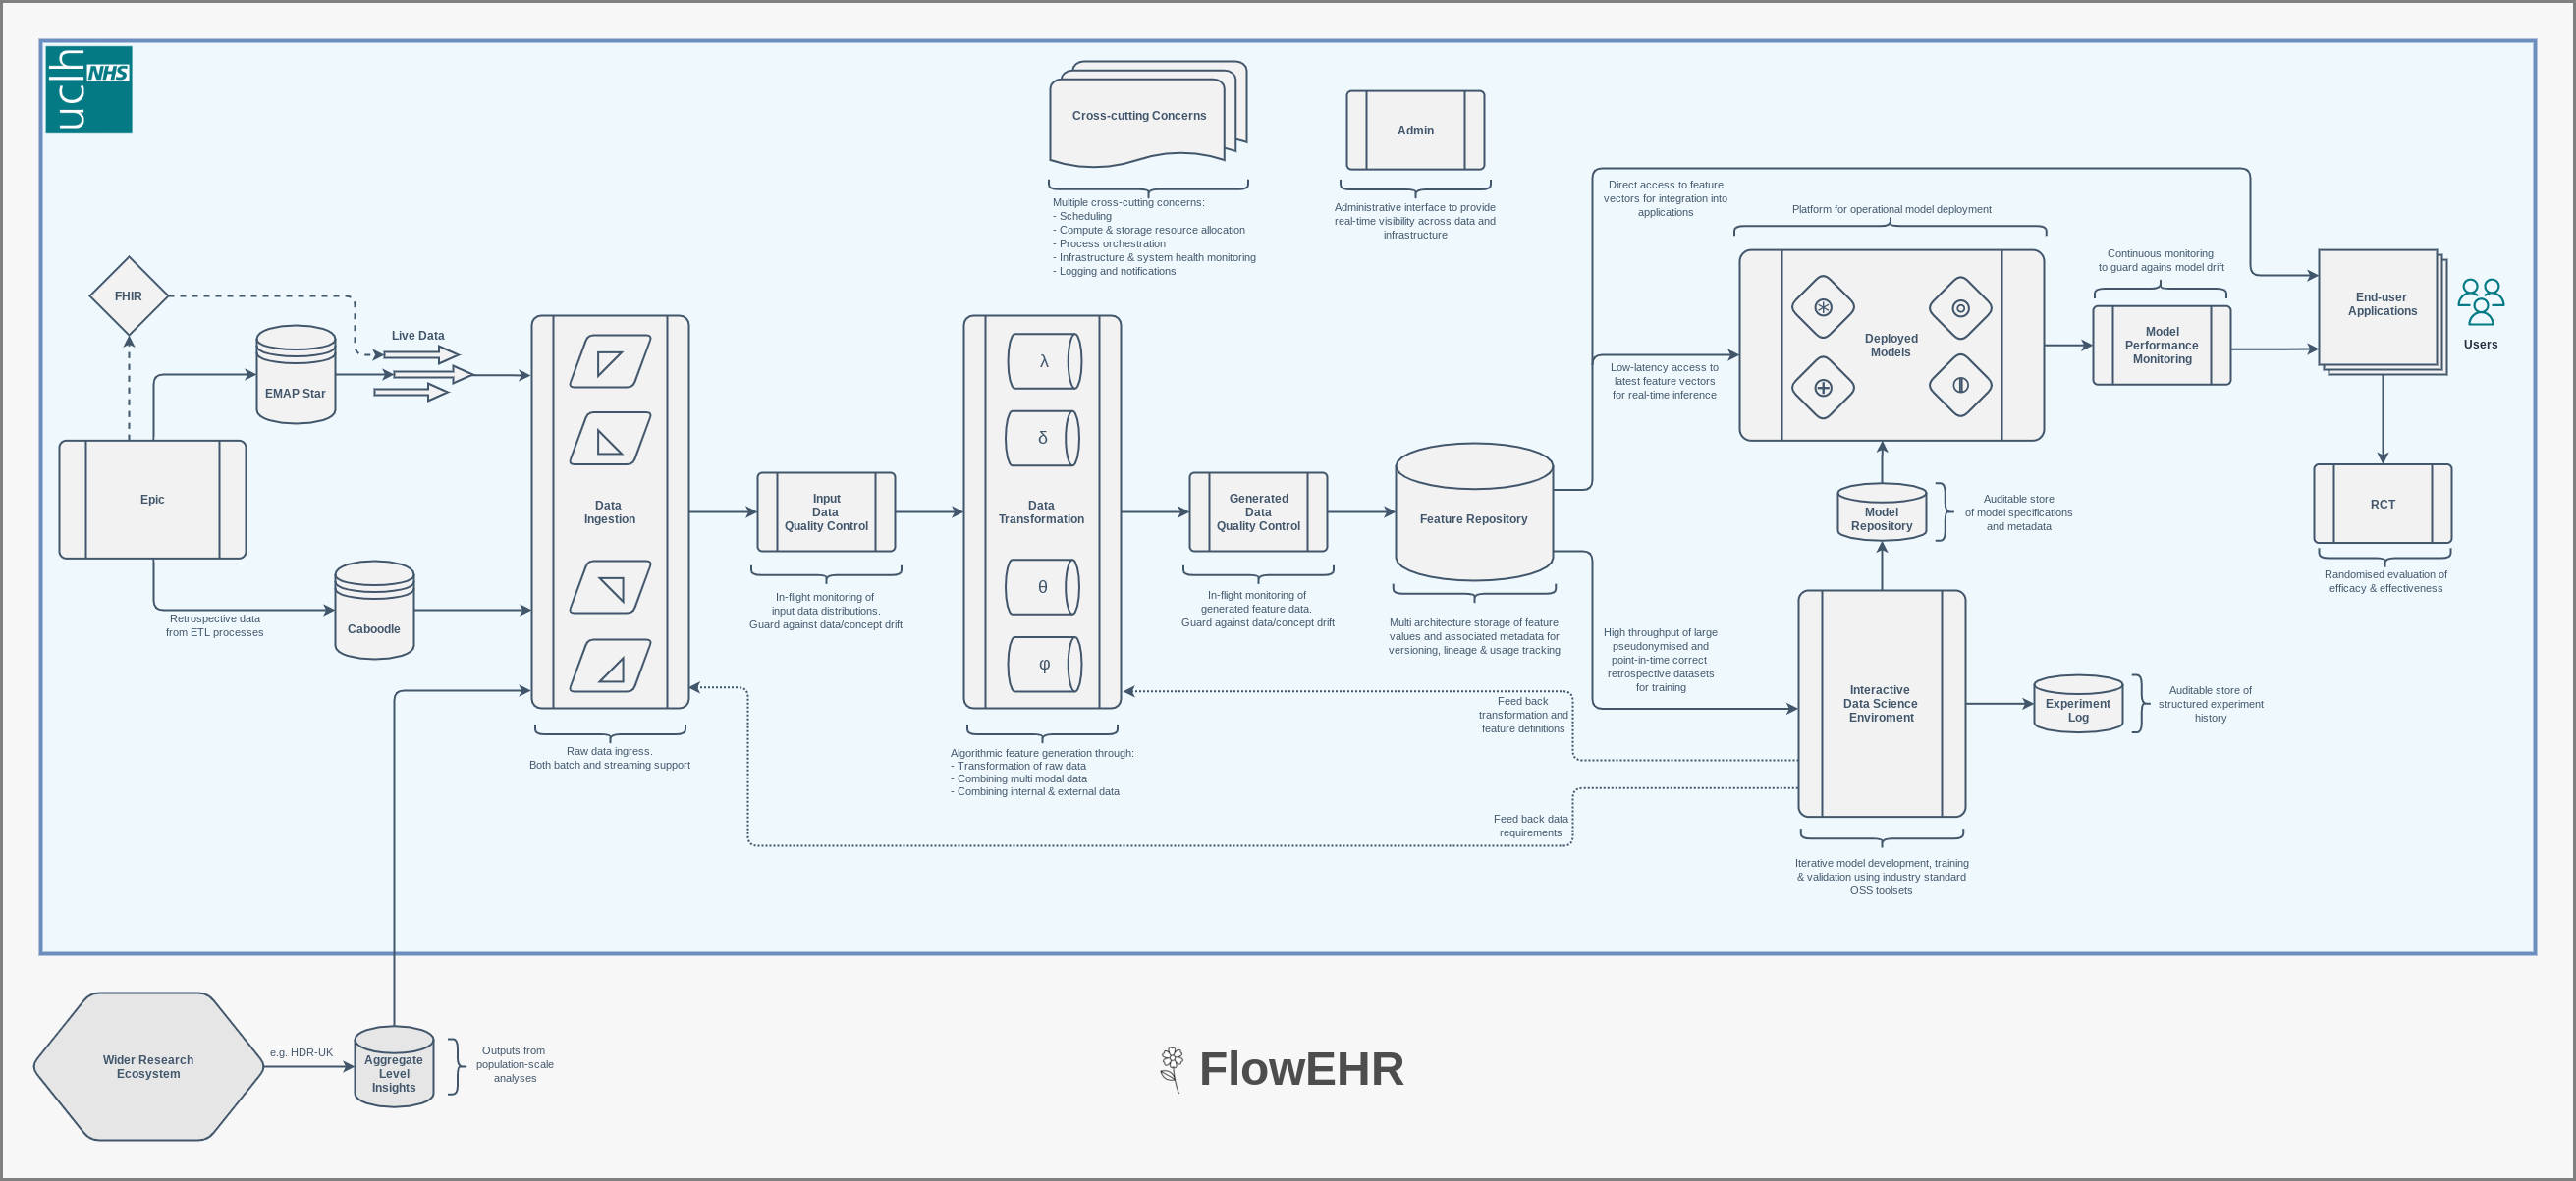
\includegraphics[width=15cm]{figs/flowehr.png}
\end{center}
\caption{
Our ML-Ops platform is called FlowEHR. Moving from left to right across the figure, the system monitors raw input data including checks for distribution shift, builds features with testable and quality controlled code, makes those features available to for both training and predictions to avoid train/serve skew, and maintains an auditable and monitored model repository.
}\label{fig:2}
\end{figure}

%%% If you are submitting a figure with subfigures please combine these into one image file with part labels integrated.
%%% If you don't add the figures in the LaTeX files, please upload them when submitting the article.
%%% Frontiers will add the figures at the end of the provisional pdf automatically
%%% The use of LaTeX coding to draw Diagrams/Figures/Structures should be avoided. They should be external callouts including graphics.



\end{document}
